\section{Introduction}

\subsection{The Role of Historical Institutions}

\begin{frame}
\frametitle{The Role of Historical Institutions}
\begin{itemize}

\item The author examine the long-run impacts of the mining mita, a forced labor system instituted by the Spanish government in Peru and Bolivia in 1573 and abolished in 1812.\\[20pt]

\item Studies find quantitative support for an impact of history on current economic outcomes \textbf {but have not focused on channels of persistence.}\\[20pt]

\item The paper use variation in the assignment of an historical institution in Peru (Mita) to identify land tenure, public goods and Market Participation as channels through which its effects persist.



\end{itemize}
\end{frame}


\begin{frame}
\frametitle{The Role of Historical Institutions (Cont)}
\begin{itemize}
\item The mita required over 200 indigenous communities to send one-seventh of their adult male population to work in the Potosí silver and Huancavelica mercury mines


\begin{center}
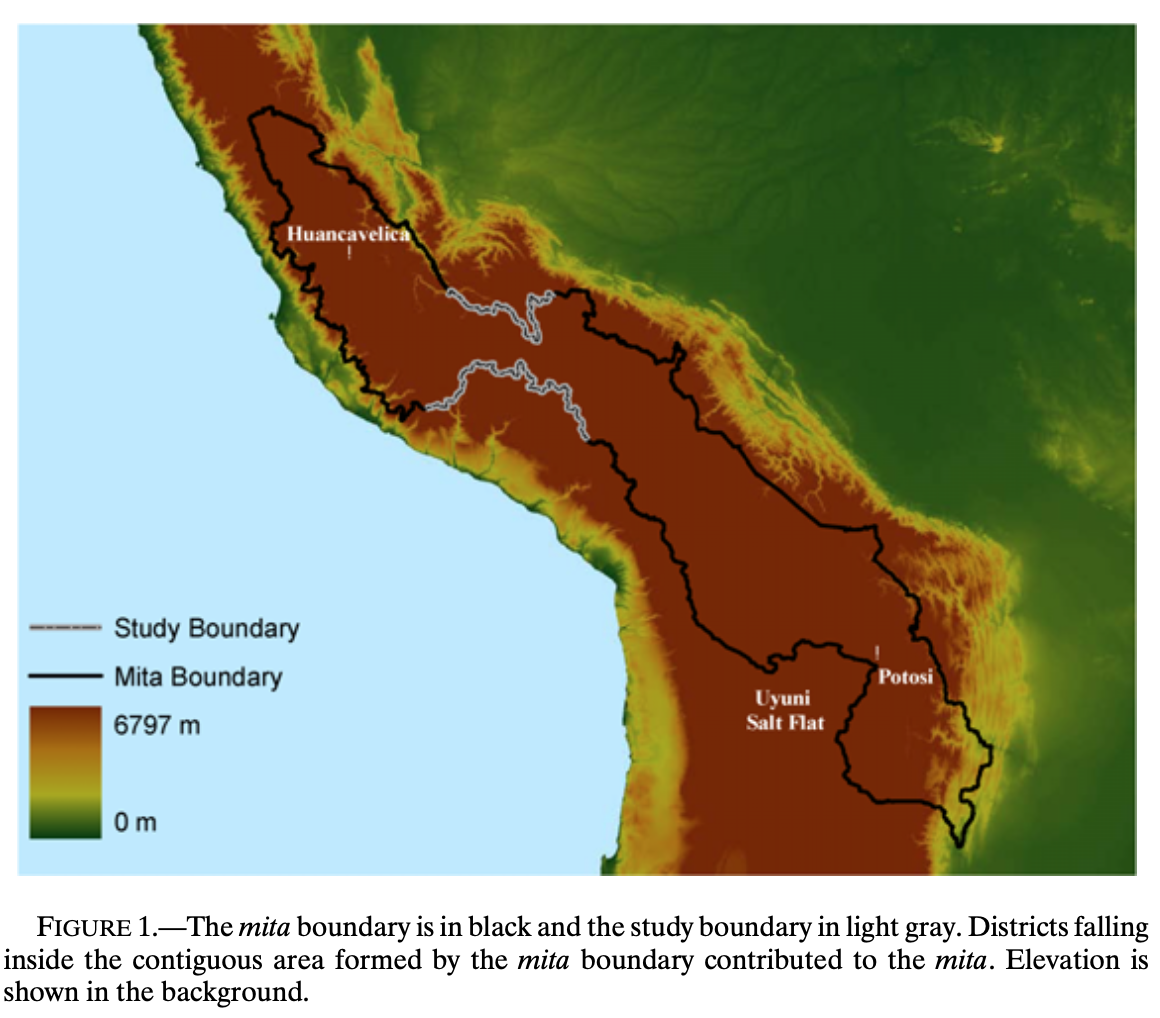
\includegraphics[width=.6\textwidth] {Peru1.png}
\end{center}




\end{itemize}


\end{frame}


\begin{frame}
\frametitle{The Role of Historical Institutions (Cont)}
\begin{itemize}

\item The paper estimate that a long- run mita effect lowers equivalent household consumption by around 25 \% in subjected districts.\\[20pt]

\item The paper also shows that the mita’s persistent impact increases childhood stunting by around 6 percent- age points in subjected districts.\\[20pt]

\item  \textbf {This support the well known hypothesis that extractive historical institutions influence long-run economic prosperity.}

\end{itemize}


\end{frame}

\begin{frame}
\frametitle{3 Channels of persistence}
\begin{itemize}

\item The haciendas developed primarily outside the mita catchment.\\[20pt]

\item The mita effect lowered education historically, and today mita districts remain less integrated into road networks.\\[20pt]

\item There are evidence that a long-run mita impact increases the prevalence of subsistence farming.\\[20pt]

\end{itemize}


\end{frame}